\documentclass[twoside]{book}

% Packages required by doxygen
\usepackage{fixltx2e}
\usepackage{calc}
\usepackage{doxygen}
\usepackage{graphicx}
\usepackage[utf8]{inputenc}
\usepackage{makeidx}
\usepackage{multicol}
\usepackage{multirow}
\PassOptionsToPackage{warn}{textcomp}
\usepackage{textcomp}
\usepackage[nointegrals]{wasysym}
\usepackage[table]{xcolor}

% NLS support packages
\usepackage[catalan]{babel}

% Font selection
\usepackage[T1]{fontenc}
\usepackage{mathptmx}
\usepackage[scaled=.90]{helvet}
\usepackage{courier}
\usepackage{amssymb}
\usepackage{sectsty}
\renewcommand{\familydefault}{\sfdefault}
\allsectionsfont{%
  \fontseries{bc}\selectfont%
  \color{darkgray}%
}
\renewcommand{\DoxyLabelFont}{%
  \fontseries{bc}\selectfont%
  \color{darkgray}%
}
\newcommand{\+}{\discretionary{\mbox{\scriptsize$\hookleftarrow$}}{}{}}

% Page & text layout
\usepackage{geometry}
\geometry{%
  a4paper,%
  top=2.5cm,%
  bottom=2.5cm,%
  left=2.5cm,%
  right=2.5cm%
}
\tolerance=750
\hfuzz=15pt
\hbadness=750
\setlength{\emergencystretch}{15pt}
\setlength{\parindent}{0cm}
\setlength{\parskip}{0.2cm}
\makeatletter
\renewcommand{\paragraph}{%
  \@startsection{paragraph}{4}{0ex}{-1.0ex}{1.0ex}{%
    \normalfont\normalsize\bfseries\SS@parafont%
  }%
}
\renewcommand{\subparagraph}{%
  \@startsection{subparagraph}{5}{0ex}{-1.0ex}{1.0ex}{%
    \normalfont\normalsize\bfseries\SS@subparafont%
  }%
}
\makeatother

% Headers & footers
\usepackage{fancyhdr}
\pagestyle{fancyplain}
\fancyhead[LE]{\fancyplain{}{\bfseries\thepage}}
\fancyhead[CE]{\fancyplain{}{}}
\fancyhead[RE]{\fancyplain{}{\bfseries\leftmark}}
\fancyhead[LO]{\fancyplain{}{\bfseries\rightmark}}
\fancyhead[CO]{\fancyplain{}{}}
\fancyhead[RO]{\fancyplain{}{\bfseries\thepage}}
\fancyfoot[LE]{\fancyplain{}{}}
\fancyfoot[CE]{\fancyplain{}{}}
\fancyfoot[RE]{\fancyplain{}{\bfseries\scriptsize Generat a Dv Mar 4 2016 17\+:19\+:45 per a Laboratori de P\+R\+O2. Especificació amb Doxygen per Doxygen }}
\fancyfoot[LO]{\fancyplain{}{\bfseries\scriptsize Generat a Dv Mar 4 2016 17\+:19\+:45 per a Laboratori de P\+R\+O2. Especificació amb Doxygen per Doxygen }}
\fancyfoot[CO]{\fancyplain{}{}}
\fancyfoot[RO]{\fancyplain{}{}}
\renewcommand{\footrulewidth}{0.4pt}
\renewcommand{\chaptermark}[1]{%
  \markboth{#1}{}%
}
\renewcommand{\sectionmark}[1]{%
  \markright{\thesection\ #1}%
}

% Indices & bibliography
\usepackage{natbib}
\usepackage[titles]{tocloft}
\setcounter{tocdepth}{3}
\setcounter{secnumdepth}{5}
\makeindex

% Hyperlinks (required, but should be loaded last)
\usepackage{ifpdf}
\ifpdf
  \usepackage[pdftex,pagebackref=true]{hyperref}
\else
  \usepackage[ps2pdf,pagebackref=true]{hyperref}
\fi
\hypersetup{%
  colorlinks=true,%
  linkcolor=blue,%
  citecolor=blue,%
  unicode%
}

% Custom commands
\newcommand{\clearemptydoublepage}{%
  \newpage{\pagestyle{empty}\cleardoublepage}%
}


%===== C O N T E N T S =====

\begin{document}

% Titlepage & ToC
\hypersetup{pageanchor=false,
             bookmarks=true,
             bookmarksnumbered=true,
             pdfencoding=unicode
            }
\pagenumbering{roman}
\begin{titlepage}
\vspace*{7cm}
\begin{center}%
{\Large Laboratori de P\+R\+O2. Especificació amb Doxygen \\[1ex]\large versió abr-\/2016 }\\
\vspace*{1cm}
{\large Generat per Doxygen 1.8.8}\\
\vspace*{0.5cm}
{\small Dv Mar 4 2016 17:19:45}\\
\end{center}
\end{titlepage}
\clearemptydoublepage
\tableofcontents
\clearemptydoublepage
\pagenumbering{arabic}
\hypersetup{pageanchor=true}

%--- Begin generated contents ---
\chapter{Exemple d'ús del Doxygen per documentar especificacions\+: classes Estudiant i Cjt\+\_\+estudiants.}
\label{index}\hypertarget{index}{}En aquest exemple es presenta un programa modular que fa servir les classes {\itshape  \hyperlink{class_estudiant}{Estudiant} } i {\itshape  \hyperlink{class_cjt__estudiants}{Cjt\+\_\+estudiants}}.

Només documentem els elements públics. Més endavant mostrarem un exemple de projecte complet. 
\chapter{Índex de Classes}
\section{Lista de clases}
Lista de las clases, estructuras, uniones e interfaces con una breve descripción\+:\begin{DoxyCompactList}
\item\contentsline{section}{\hyperlink{class_cubeta}{Cubeta} \\*Representa una cubeta de ropa }{\pageref{class_cubeta}}{}
\item\contentsline{section}{\hyperlink{class_lavadora}{Lavadora} \\*Representa una lavadora }{\pageref{class_lavadora}}{}
\item\contentsline{section}{\hyperlink{class_prenda}{Prenda} \\*Representa una prenda de ropa con atributos peso y color }{\pageref{class_prenda}}{}
\end{DoxyCompactList}

\chapter{Índex de Fitxers}
\section{Llista dels Fitxers}
Aquesta és la llista de tots els fitxers acompanyats amb breus descripcions\+:\begin{DoxyCompactList}
\item\contentsline{section}{\hyperlink{_cjt__estudiants_8hh}{Cjt\+\_\+estudiants.\+hh} \\*Especificació de la classe \hyperlink{class_cjt__estudiants}{Cjt\+\_\+estudiants} }{\pageref{_cjt__estudiants_8hh}}{}
\item\contentsline{section}{\hyperlink{_estudiant_8hh}{Estudiant.\+hh} \\*Especificació de la classe \hyperlink{class_estudiant}{Estudiant} }{\pageref{_estudiant_8hh}}{}
\item\contentsline{section}{\hyperlink{pro2__doxygen_8cc}{pro2\+\_\+doxygen.\+cc} }{\pageref{pro2__doxygen_8cc}}{}
\end{DoxyCompactList}

\chapter{Documentació de les Classes}
\hypertarget{class_cjt__estudiants}{\section{Referència de la Classe Cjt\+\_\+estudiants}
\label{class_cjt__estudiants}\index{Cjt\+\_\+estudiants@{Cjt\+\_\+estudiants}}
}


Representa un conjunt d'estudiants ordenat per D\+N\+I. Es poden consultar i modificar els seus elements (de tipus \hyperlink{class_estudiant}{Estudiant}) donat un estudiant concret o per posicio a l'ordre.  


\subsection*{Mètodes públics}
\begin{DoxyCompactItemize}
\item 
\hyperlink{class_cjt__estudiants_a31ffe72cadcf58d82c8b9f6659c56e7a}{Cjt\+\_\+estudiants} ()
\begin{DoxyCompactList}\small\item\em Creadora per defecte. \end{DoxyCompactList}\item 
void \hyperlink{class_cjt__estudiants_a8724107ebfbe917c45906f7e6d510867}{afegir\+\_\+estudiant} (const \hyperlink{class_estudiant}{Estudiant} \&est)
\begin{DoxyCompactList}\small\item\em Afegeix un estudiant a un conjunt. \end{DoxyCompactList}\item 
void \hyperlink{class_cjt__estudiants_ae5b64b1e3ea3587e00a32e6fbeae2e7c}{modificar\+\_\+estudiant} (const \hyperlink{class_estudiant}{Estudiant} \&est)
\begin{DoxyCompactList}\small\item\em Modifica un estudiant dins d'un conjunt. \end{DoxyCompactList}\item 
void \hyperlink{class_cjt__estudiants_a18590359c8f8537aa38711febf6c8bbf}{modificar\+\_\+iessim} (int i, const \hyperlink{class_estudiant}{Estudiant} \&est)
\begin{DoxyCompactList}\small\item\em Modifica l'i-\/esim estudiant dins d'un conjunt. \end{DoxyCompactList}\item 
int \hyperlink{class_cjt__estudiants_a8b25d97f6e061b2986e18c67a0d49f73}{mida} () const 
\begin{DoxyCompactList}\small\item\em Consulta la mida d'un conjunt d'estudiants. \end{DoxyCompactList}\item 
bool \hyperlink{class_cjt__estudiants_ada47d1e52a6910bb0b1ce21090f8c855}{existeix\+\_\+estudiant} (int dni) const 
\begin{DoxyCompactList}\small\item\em Cerca d'un estudiant a un conjunt. \end{DoxyCompactList}\item 
\hyperlink{class_estudiant}{Estudiant} \hyperlink{class_cjt__estudiants_a90a7bb740b5b14c1038cdfe4b3468674}{consultar\+\_\+estudiant} (int dni) const 
\begin{DoxyCompactList}\small\item\em Consulta d'un estudiant a un conjunt. \end{DoxyCompactList}\item 
\hyperlink{class_estudiant}{Estudiant} \hyperlink{class_cjt__estudiants_a1c598f56d048d036df3ba0afd6fc5ea9}{consultar\+\_\+iessim} (int i) const 
\begin{DoxyCompactList}\small\item\em Consulta de l'estudiant i-\/esim d'un conjunt. \end{DoxyCompactList}\item 
void \hyperlink{class_cjt__estudiants_aa24c2d4c36167b2b810ab459435b67a8}{llegir} ()
\begin{DoxyCompactList}\small\item\em Operacio de lectura. \end{DoxyCompactList}\item 
void \hyperlink{class_cjt__estudiants_a80ca07a3078ae102740a1f1a152ed0a1}{escriure} () const 
\begin{DoxyCompactList}\small\item\em Operacio d'escriptura. \end{DoxyCompactList}\end{DoxyCompactItemize}
\subsection*{Mètodes Públics Estàtics}
\begin{DoxyCompactItemize}
\item 
static int \hyperlink{class_cjt__estudiants_a171fdff58b408ccbf647ab594b5eafa4}{mida\+\_\+maxima} ()
\begin{DoxyCompactList}\small\item\em Consulta de la mida maxima de la classe \hyperlink{class_cjt__estudiants}{Cjt\+\_\+estudiants}. \end{DoxyCompactList}\end{DoxyCompactItemize}


\subsection{Descripció Detallada}
Representa un conjunt d'estudiants ordenat per D\+N\+I. Es poden consultar i modificar els seus elements (de tipus \hyperlink{class_estudiant}{Estudiant}) donat un estudiant concret o per posicio a l'ordre. 

Definició a la línia 21 del fitxer Cjt\+\_\+estudiants.\+hh.



\subsection{Documentació del Constructor i el Destructor}
\hypertarget{class_cjt__estudiants_a31ffe72cadcf58d82c8b9f6659c56e7a}{\index{Cjt\+\_\+estudiants@{Cjt\+\_\+estudiants}!Cjt\+\_\+estudiants@{Cjt\+\_\+estudiants}}
\index{Cjt\+\_\+estudiants@{Cjt\+\_\+estudiants}!Cjt\+\_\+estudiants@{Cjt\+\_\+estudiants}}
\subsubsection[{Cjt\+\_\+estudiants}]{\setlength{\rightskip}{0pt plus 5cm}Cjt\+\_\+estudiants\+::\+Cjt\+\_\+estudiants (
\begin{DoxyParamCaption}
{}
\end{DoxyParamCaption}
)}}\label{class_cjt__estudiants_a31ffe72cadcf58d82c8b9f6659c56e7a}


Creadora per defecte. 

S'executa automaticament al declarar \hyperlink{class_cjt__estudiants}{Cjt\+\_\+estudiants} c; \begin{DoxyPrecond}{Precondició}
cert 
\end{DoxyPrecond}
\begin{DoxyPostcond}{Postcondició}
el resultat es un conjunt d'estudiants buit 
\end{DoxyPostcond}


\subsection{Documentació de les Funcions Membre}
\hypertarget{class_cjt__estudiants_a8724107ebfbe917c45906f7e6d510867}{\index{Cjt\+\_\+estudiants@{Cjt\+\_\+estudiants}!afegir\+\_\+estudiant@{afegir\+\_\+estudiant}}
\index{afegir\+\_\+estudiant@{afegir\+\_\+estudiant}!Cjt\+\_\+estudiants@{Cjt\+\_\+estudiants}}
\subsubsection[{afegir\+\_\+estudiant}]{\setlength{\rightskip}{0pt plus 5cm}void Cjt\+\_\+estudiants\+::afegir\+\_\+estudiant (
\begin{DoxyParamCaption}
\item[{const {\bf Estudiant} \&}]{est}
\end{DoxyParamCaption}
)}}\label{class_cjt__estudiants_a8724107ebfbe917c45906f7e6d510867}


Afegeix un estudiant a un conjunt. 

\begin{DoxyPrecond}{Precondició}
el parametre implicit no conte cap estudiant amb el D\+N\+I d'est; el nombre d'estudiants del p.\+i. es mes petit que la mida maxima permesa 
\end{DoxyPrecond}
\begin{DoxyPostcond}{Postcondició}
s'ha afegit l'estudiant est al parametre implicit 
\end{DoxyPostcond}
\hypertarget{class_cjt__estudiants_ae5b64b1e3ea3587e00a32e6fbeae2e7c}{\index{Cjt\+\_\+estudiants@{Cjt\+\_\+estudiants}!modificar\+\_\+estudiant@{modificar\+\_\+estudiant}}
\index{modificar\+\_\+estudiant@{modificar\+\_\+estudiant}!Cjt\+\_\+estudiants@{Cjt\+\_\+estudiants}}
\subsubsection[{modificar\+\_\+estudiant}]{\setlength{\rightskip}{0pt plus 5cm}void Cjt\+\_\+estudiants\+::modificar\+\_\+estudiant (
\begin{DoxyParamCaption}
\item[{const {\bf Estudiant} \&}]{est}
\end{DoxyParamCaption}
)}}\label{class_cjt__estudiants_ae5b64b1e3ea3587e00a32e6fbeae2e7c}


Modifica un estudiant dins d'un conjunt. 

\begin{DoxyPrecond}{Precondició}
existeix un estudiant al parametre implicit amb el D\+N\+I d'est 
\end{DoxyPrecond}
\begin{DoxyPostcond}{Postcondició}
l'estudiant del parametre implicit original amb el dni d'est, ha quedat substituit per est 
\end{DoxyPostcond}
\hypertarget{class_cjt__estudiants_a18590359c8f8537aa38711febf6c8bbf}{\index{Cjt\+\_\+estudiants@{Cjt\+\_\+estudiants}!modificar\+\_\+iessim@{modificar\+\_\+iessim}}
\index{modificar\+\_\+iessim@{modificar\+\_\+iessim}!Cjt\+\_\+estudiants@{Cjt\+\_\+estudiants}}
\subsubsection[{modificar\+\_\+iessim}]{\setlength{\rightskip}{0pt plus 5cm}void Cjt\+\_\+estudiants\+::modificar\+\_\+iessim (
\begin{DoxyParamCaption}
\item[{int}]{i, }
\item[{const {\bf Estudiant} \&}]{est}
\end{DoxyParamCaption}
)}}\label{class_cjt__estudiants_a18590359c8f8537aa38711febf6c8bbf}


Modifica l'i-\/esim estudiant dins d'un conjunt. 

\begin{DoxyPrecond}{Precondició}
1 $<$= i $<$= \hyperlink{class_cjt__estudiants_a8b25d97f6e061b2986e18c67a0d49f73}{mida()}, l'element i-\/esim del conjunt en ordre creixent per D\+N\+I conte un estudiant amb el mateix D\+N\+I que est 
\end{DoxyPrecond}
\begin{DoxyPostcond}{Postcondició}
l'estudiant est ha substituit l'estudiant i-\/esim del parametre implicit 
\end{DoxyPostcond}
\hypertarget{class_cjt__estudiants_a8b25d97f6e061b2986e18c67a0d49f73}{\index{Cjt\+\_\+estudiants@{Cjt\+\_\+estudiants}!mida@{mida}}
\index{mida@{mida}!Cjt\+\_\+estudiants@{Cjt\+\_\+estudiants}}
\subsubsection[{mida}]{\setlength{\rightskip}{0pt plus 5cm}int Cjt\+\_\+estudiants\+::mida (
\begin{DoxyParamCaption}
{}
\end{DoxyParamCaption}
) const}}\label{class_cjt__estudiants_a8b25d97f6e061b2986e18c67a0d49f73}


Consulta la mida d'un conjunt d'estudiants. 

\begin{DoxyPrecond}{Precondició}
cert 
\end{DoxyPrecond}
\begin{DoxyPostcond}{Postcondició}
el resultat es la mida del parametre implicit 
\end{DoxyPostcond}
\hypertarget{class_cjt__estudiants_a171fdff58b408ccbf647ab594b5eafa4}{\index{Cjt\+\_\+estudiants@{Cjt\+\_\+estudiants}!mida\+\_\+maxima@{mida\+\_\+maxima}}
\index{mida\+\_\+maxima@{mida\+\_\+maxima}!Cjt\+\_\+estudiants@{Cjt\+\_\+estudiants}}
\subsubsection[{mida\+\_\+maxima}]{\setlength{\rightskip}{0pt plus 5cm}static int Cjt\+\_\+estudiants\+::mida\+\_\+maxima (
\begin{DoxyParamCaption}
{}
\end{DoxyParamCaption}
)\hspace{0.3cm}{\ttfamily [static]}}}\label{class_cjt__estudiants_a171fdff58b408ccbf647ab594b5eafa4}


Consulta de la mida maxima de la classe \hyperlink{class_cjt__estudiants}{Cjt\+\_\+estudiants}. 

\begin{DoxyPrecond}{Precondició}
cert 
\end{DoxyPrecond}
\begin{DoxyPostcond}{Postcondició}
el resultat es la mida maxima dels elements de la classe 
\end{DoxyPostcond}
\hypertarget{class_cjt__estudiants_ada47d1e52a6910bb0b1ce21090f8c855}{\index{Cjt\+\_\+estudiants@{Cjt\+\_\+estudiants}!existeix\+\_\+estudiant@{existeix\+\_\+estudiant}}
\index{existeix\+\_\+estudiant@{existeix\+\_\+estudiant}!Cjt\+\_\+estudiants@{Cjt\+\_\+estudiants}}
\subsubsection[{existeix\+\_\+estudiant}]{\setlength{\rightskip}{0pt plus 5cm}bool Cjt\+\_\+estudiants\+::existeix\+\_\+estudiant (
\begin{DoxyParamCaption}
\item[{int}]{dni}
\end{DoxyParamCaption}
) const}}\label{class_cjt__estudiants_ada47d1e52a6910bb0b1ce21090f8c855}


Cerca d'un estudiant a un conjunt. 

\begin{DoxyPrecond}{Precondició}
dni $>$= 0 
\end{DoxyPrecond}
\begin{DoxyPostcond}{Postcondició}
el resultat indica si existeix un estudiant al parametre implicit amb D\+N\+I = dni 
\end{DoxyPostcond}
\hypertarget{class_cjt__estudiants_a90a7bb740b5b14c1038cdfe4b3468674}{\index{Cjt\+\_\+estudiants@{Cjt\+\_\+estudiants}!consultar\+\_\+estudiant@{consultar\+\_\+estudiant}}
\index{consultar\+\_\+estudiant@{consultar\+\_\+estudiant}!Cjt\+\_\+estudiants@{Cjt\+\_\+estudiants}}
\subsubsection[{consultar\+\_\+estudiant}]{\setlength{\rightskip}{0pt plus 5cm}{\bf Estudiant} Cjt\+\_\+estudiants\+::consultar\+\_\+estudiant (
\begin{DoxyParamCaption}
\item[{int}]{dni}
\end{DoxyParamCaption}
) const}}\label{class_cjt__estudiants_a90a7bb740b5b14c1038cdfe4b3468674}


Consulta d'un estudiant a un conjunt. 

\begin{DoxyPrecond}{Precondició}
existeix un estudiant al parametre implicit amb D\+N\+I = dni 
\end{DoxyPrecond}
\begin{DoxyPostcond}{Postcondició}
el resultat es l'estudiant amb D\+N\+I = dni que conte el parametre implicit 
\end{DoxyPostcond}
\hypertarget{class_cjt__estudiants_a1c598f56d048d036df3ba0afd6fc5ea9}{\index{Cjt\+\_\+estudiants@{Cjt\+\_\+estudiants}!consultar\+\_\+iessim@{consultar\+\_\+iessim}}
\index{consultar\+\_\+iessim@{consultar\+\_\+iessim}!Cjt\+\_\+estudiants@{Cjt\+\_\+estudiants}}
\subsubsection[{consultar\+\_\+iessim}]{\setlength{\rightskip}{0pt plus 5cm}{\bf Estudiant} Cjt\+\_\+estudiants\+::consultar\+\_\+iessim (
\begin{DoxyParamCaption}
\item[{int}]{i}
\end{DoxyParamCaption}
) const}}\label{class_cjt__estudiants_a1c598f56d048d036df3ba0afd6fc5ea9}


Consulta de l'estudiant i-\/esim d'un conjunt. 

\begin{DoxyPrecond}{Precondició}
1 $<$= i $<$= \hyperlink{class_cjt__estudiants_a8b25d97f6e061b2986e18c67a0d49f73}{mida()} 
\end{DoxyPrecond}
\begin{DoxyPostcond}{Postcondició}
el resultat es l'estudiant i-\/essim del parametre implicit en ordre creixent per D\+N\+I 
\end{DoxyPostcond}
\hypertarget{class_cjt__estudiants_aa24c2d4c36167b2b810ab459435b67a8}{\index{Cjt\+\_\+estudiants@{Cjt\+\_\+estudiants}!llegir@{llegir}}
\index{llegir@{llegir}!Cjt\+\_\+estudiants@{Cjt\+\_\+estudiants}}
\subsubsection[{llegir}]{\setlength{\rightskip}{0pt plus 5cm}void Cjt\+\_\+estudiants\+::llegir (
\begin{DoxyParamCaption}
{}
\end{DoxyParamCaption}
)}}\label{class_cjt__estudiants_aa24c2d4c36167b2b810ab459435b67a8}


Operacio de lectura. 

\begin{DoxyPrecond}{Precondició}
estan preparats al canal estandard d'entrada un enter (entre 0 i la mida maxima permesa per a la classe), que representa el nombre d'elements que llegirem, i les dades de tal nombre d'estudiants diferents 
\end{DoxyPrecond}
\begin{DoxyPostcond}{Postcondició}
el parametre implicit conte el conjunt d'estudiants llegits del canal estandard d'entrada 
\end{DoxyPostcond}
\hypertarget{class_cjt__estudiants_a80ca07a3078ae102740a1f1a152ed0a1}{\index{Cjt\+\_\+estudiants@{Cjt\+\_\+estudiants}!escriure@{escriure}}
\index{escriure@{escriure}!Cjt\+\_\+estudiants@{Cjt\+\_\+estudiants}}
\subsubsection[{escriure}]{\setlength{\rightskip}{0pt plus 5cm}void Cjt\+\_\+estudiants\+::escriure (
\begin{DoxyParamCaption}
{}
\end{DoxyParamCaption}
) const}}\label{class_cjt__estudiants_a80ca07a3078ae102740a1f1a152ed0a1}


Operacio d'escriptura. 

\begin{DoxyPrecond}{Precondició}
cert 
\end{DoxyPrecond}
\begin{DoxyPostcond}{Postcondició}
s'han escrit pel canal estandard de sortida els estudiants del parametre implicit en ordre ascendent per D\+N\+I 
\end{DoxyPostcond}


La documentació d'aquesta classe es va generar a partir del següent fitxer\+:\begin{DoxyCompactItemize}
\item 
\hyperlink{_cjt__estudiants_8hh}{Cjt\+\_\+estudiants.\+hh}\end{DoxyCompactItemize}

\hypertarget{class_estudiant}{\section{Referència de la Classe Estudiant}
\label{class_estudiant}\index{Estudiant@{Estudiant}}
}


Representa un estudiant amb D\+N\+I, que pot tenir nota.  


\subsection*{Mètodes públics}
\begin{DoxyCompactItemize}
\item 
\hyperlink{class_estudiant_a88f7f46dd946fef9f7a71fdc608afd16}{Estudiant} ()
\begin{DoxyCompactList}\small\item\em Creadora per defecte. \end{DoxyCompactList}\item 
\hyperlink{class_estudiant_ae0a9ebffe2ff8fb6cecc15a909206a1b}{Estudiant} (int dni)
\begin{DoxyCompactList}\small\item\em Creadora amb D\+N\+I. \end{DoxyCompactList}\item 
void \hyperlink{class_estudiant_a8a2186560dce4ccfc5922d2c98f21305}{afegir\+\_\+nota} (double nota)
\begin{DoxyCompactList}\small\item\em Afegeix una nota a un estudiant sense nota. \end{DoxyCompactList}\item 
void \hyperlink{class_estudiant_a5d5eded678c16a864f22477d401a56af}{modificar\+\_\+nota} (double nota)
\begin{DoxyCompactList}\small\item\em Modifica la nota d'un estudiant amb nota. \end{DoxyCompactList}\item 
int \hyperlink{class_estudiant_a5b292568ec470cb27bf41a0f097341f1}{consultar\+\_\+\+D\+N\+I} () const 
\begin{DoxyCompactList}\small\item\em Consulta del D\+N\+I d'un estudiant. \end{DoxyCompactList}\item 
double \hyperlink{class_estudiant_a0f5562a2dd1d17bac9671fe2caf2dbf7}{consultar\+\_\+nota} () const 
\begin{DoxyCompactList}\small\item\em Consulta de ls nota d'un estudiant. \end{DoxyCompactList}\item 
bool \hyperlink{class_estudiant_a237691a50419cc2bd000e8b538b17c1b}{te\+\_\+nota} () const 
\begin{DoxyCompactList}\small\item\em Comprovació de la nota d'un estudiant. \end{DoxyCompactList}\item 
void \hyperlink{class_estudiant_af5c4883975828647dfb5ffc6735740e6}{llegir} ()
\begin{DoxyCompactList}\small\item\em Operació de lectura. \end{DoxyCompactList}\item 
void \hyperlink{class_estudiant_a494ffdc9c41b9f7d97c3cc40f3d1f482}{escriure} () const 
\begin{DoxyCompactList}\small\item\em Operació d'escriptura. \end{DoxyCompactList}\end{DoxyCompactItemize}
\subsection*{Mètodes Públics Estàtics}
\begin{DoxyCompactItemize}
\item 
static double \hyperlink{class_estudiant_a5df5eed414c87a2a1c2efa4194633afd}{nota\+\_\+maxima} ()
\begin{DoxyCompactList}\small\item\em Consulta de la nota màxima de la classe \hyperlink{class_estudiant}{Estudiant}. \end{DoxyCompactList}\end{DoxyCompactItemize}


\subsection{Descripció Detallada}
Representa un estudiant amb D\+N\+I, que pot tenir nota. 

Els D\+N\+I vàlids són enters no negatius. Les notes vàlides son les de l'interval 0..\hyperlink{class_estudiant_a5df5eed414c87a2a1c2efa4194633afd}{nota\+\_\+maxima()} 

Definició a la línia 13 del fitxer Estudiant.\+hh.



\subsection{Documentació del Constructor i el Destructor}
\hypertarget{class_estudiant_a88f7f46dd946fef9f7a71fdc608afd16}{\index{Estudiant@{Estudiant}!Estudiant@{Estudiant}}
\index{Estudiant@{Estudiant}!Estudiant@{Estudiant}}
\subsubsection[{Estudiant}]{\setlength{\rightskip}{0pt plus 5cm}Estudiant\+::\+Estudiant (
\begin{DoxyParamCaption}
{}
\end{DoxyParamCaption}
)}}\label{class_estudiant_a88f7f46dd946fef9f7a71fdc608afd16}


Creadora per defecte. 

S'executa automáticament al declarar \hyperlink{class_estudiant}{Estudiant} e; \begin{DoxyPrecond}{Precondició}
cert 
\end{DoxyPrecond}
\begin{DoxyPostcond}{Postcondició}
el resultat es un estudiant amb D\+N\+I = 0 i sense nota 
\end{DoxyPostcond}
\hypertarget{class_estudiant_ae0a9ebffe2ff8fb6cecc15a909206a1b}{\index{Estudiant@{Estudiant}!Estudiant@{Estudiant}}
\index{Estudiant@{Estudiant}!Estudiant@{Estudiant}}
\subsubsection[{Estudiant}]{\setlength{\rightskip}{0pt plus 5cm}Estudiant\+::\+Estudiant (
\begin{DoxyParamCaption}
\item[{int}]{dni}
\end{DoxyParamCaption}
)}}\label{class_estudiant_ae0a9ebffe2ff8fb6cecc15a909206a1b}


Creadora amb D\+N\+I. 

S'executa automáticament al declarar \hyperlink{class_estudiant}{Estudiant} e2(e1);. \begin{DoxyPrecond}{Precondició}
cert 
\end{DoxyPrecond}
\begin{DoxyPostcond}{Postcondició}
el resultat es un estudiant amb D\+N\+I = dni i sense nota 
\end{DoxyPostcond}


\subsection{Documentació de les Funcions Membre}
\hypertarget{class_estudiant_a8a2186560dce4ccfc5922d2c98f21305}{\index{Estudiant@{Estudiant}!afegir\+\_\+nota@{afegir\+\_\+nota}}
\index{afegir\+\_\+nota@{afegir\+\_\+nota}!Estudiant@{Estudiant}}
\subsubsection[{afegir\+\_\+nota}]{\setlength{\rightskip}{0pt plus 5cm}void Estudiant\+::afegir\+\_\+nota (
\begin{DoxyParamCaption}
\item[{double}]{nota}
\end{DoxyParamCaption}
)}}\label{class_estudiant_a8a2186560dce4ccfc5922d2c98f21305}


Afegeix una nota a un estudiant sense nota. 

\begin{DoxyPrecond}{Precondició}
el parametre implicit no te nota, 0 $<$= {\itshape nota} $<$= \hyperlink{class_estudiant_a5df5eed414c87a2a1c2efa4194633afd}{nota\+\_\+maxima()} 
\end{DoxyPrecond}
\begin{DoxyPostcond}{Postcondició}
la nota del parametre implicit passa a ser {\itshape nota} 
\end{DoxyPostcond}
\hypertarget{class_estudiant_a5d5eded678c16a864f22477d401a56af}{\index{Estudiant@{Estudiant}!modificar\+\_\+nota@{modificar\+\_\+nota}}
\index{modificar\+\_\+nota@{modificar\+\_\+nota}!Estudiant@{Estudiant}}
\subsubsection[{modificar\+\_\+nota}]{\setlength{\rightskip}{0pt plus 5cm}void Estudiant\+::modificar\+\_\+nota (
\begin{DoxyParamCaption}
\item[{double}]{nota}
\end{DoxyParamCaption}
)}}\label{class_estudiant_a5d5eded678c16a864f22477d401a56af}


Modifica la nota d'un estudiant amb nota. 

\begin{DoxyPrecond}{Precondició}
el parametre implicit te nota, 0 $<$= {\itshape nota} $<$= \hyperlink{class_estudiant_a5df5eed414c87a2a1c2efa4194633afd}{nota\+\_\+maxima()} 
\end{DoxyPrecond}
\begin{DoxyPostcond}{Postcondició}
la nota del parametre implicit passa a ser {\itshape nota} 
\end{DoxyPostcond}
\hypertarget{class_estudiant_a5b292568ec470cb27bf41a0f097341f1}{\index{Estudiant@{Estudiant}!consultar\+\_\+\+D\+N\+I@{consultar\+\_\+\+D\+N\+I}}
\index{consultar\+\_\+\+D\+N\+I@{consultar\+\_\+\+D\+N\+I}!Estudiant@{Estudiant}}
\subsubsection[{consultar\+\_\+\+D\+N\+I}]{\setlength{\rightskip}{0pt plus 5cm}int Estudiant\+::consultar\+\_\+\+D\+N\+I (
\begin{DoxyParamCaption}
{}
\end{DoxyParamCaption}
) const}}\label{class_estudiant_a5b292568ec470cb27bf41a0f097341f1}


Consulta del D\+N\+I d'un estudiant. 

\begin{DoxyPrecond}{Precondició}
cert 
\end{DoxyPrecond}
\begin{DoxyPostcond}{Postcondició}
el resultat es el D\+N\+I del parametre implicit 
\end{DoxyPostcond}
\hypertarget{class_estudiant_a0f5562a2dd1d17bac9671fe2caf2dbf7}{\index{Estudiant@{Estudiant}!consultar\+\_\+nota@{consultar\+\_\+nota}}
\index{consultar\+\_\+nota@{consultar\+\_\+nota}!Estudiant@{Estudiant}}
\subsubsection[{consultar\+\_\+nota}]{\setlength{\rightskip}{0pt plus 5cm}double Estudiant\+::consultar\+\_\+nota (
\begin{DoxyParamCaption}
{}
\end{DoxyParamCaption}
) const}}\label{class_estudiant_a0f5562a2dd1d17bac9671fe2caf2dbf7}


Consulta de ls nota d'un estudiant. 

\begin{DoxyPrecond}{Precondició}
el parametre implicit te nota 
\end{DoxyPrecond}
\begin{DoxyPostcond}{Postcondició}
el resultat es la nota del parametre implicit 
\end{DoxyPostcond}
\hypertarget{class_estudiant_a5df5eed414c87a2a1c2efa4194633afd}{\index{Estudiant@{Estudiant}!nota\+\_\+maxima@{nota\+\_\+maxima}}
\index{nota\+\_\+maxima@{nota\+\_\+maxima}!Estudiant@{Estudiant}}
\subsubsection[{nota\+\_\+maxima}]{\setlength{\rightskip}{0pt plus 5cm}static double Estudiant\+::nota\+\_\+maxima (
\begin{DoxyParamCaption}
{}
\end{DoxyParamCaption}
)\hspace{0.3cm}{\ttfamily [static]}}}\label{class_estudiant_a5df5eed414c87a2a1c2efa4194633afd}


Consulta de la nota màxima de la classe \hyperlink{class_estudiant}{Estudiant}. 

\begin{DoxyPrecond}{Precondició}
cert 
\end{DoxyPrecond}
\begin{DoxyPostcond}{Postcondició}
el resultat es la nota maxima dels elements de la classe 
\end{DoxyPostcond}
\hypertarget{class_estudiant_a237691a50419cc2bd000e8b538b17c1b}{\index{Estudiant@{Estudiant}!te\+\_\+nota@{te\+\_\+nota}}
\index{te\+\_\+nota@{te\+\_\+nota}!Estudiant@{Estudiant}}
\subsubsection[{te\+\_\+nota}]{\setlength{\rightskip}{0pt plus 5cm}bool Estudiant\+::te\+\_\+nota (
\begin{DoxyParamCaption}
{}
\end{DoxyParamCaption}
) const}}\label{class_estudiant_a237691a50419cc2bd000e8b538b17c1b}


Comprovació de la nota d'un estudiant. 

\begin{DoxyPrecond}{Precondició}
cert 
\end{DoxyPrecond}
\begin{DoxyPostcond}{Postcondició}
el resultat indica si el parametre implicit te nota o no 
\end{DoxyPostcond}
\hypertarget{class_estudiant_af5c4883975828647dfb5ffc6735740e6}{\index{Estudiant@{Estudiant}!llegir@{llegir}}
\index{llegir@{llegir}!Estudiant@{Estudiant}}
\subsubsection[{llegir}]{\setlength{\rightskip}{0pt plus 5cm}void Estudiant\+::llegir (
\begin{DoxyParamCaption}
{}
\end{DoxyParamCaption}
)}}\label{class_estudiant_af5c4883975828647dfb5ffc6735740e6}


Operació de lectura. 

\begin{DoxyPrecond}{Precondició}
hi ha preparats al canal estandard d'entrada un enter no negatiu i un double 
\end{DoxyPrecond}
\begin{DoxyPostcond}{Postcondició}
el parametre implicit passa a tenir els atributs llegits del canal estandard d'entrada; si el double no pertany a l'interval \mbox{[}0..\hyperlink{class_estudiant_a5df5eed414c87a2a1c2efa4194633afd}{nota\+\_\+maxima()}\mbox{]}, el p.\+i. es queda sense nota 
\end{DoxyPostcond}
\hypertarget{class_estudiant_a494ffdc9c41b9f7d97c3cc40f3d1f482}{\index{Estudiant@{Estudiant}!escriure@{escriure}}
\index{escriure@{escriure}!Estudiant@{Estudiant}}
\subsubsection[{escriure}]{\setlength{\rightskip}{0pt plus 5cm}void Estudiant\+::escriure (
\begin{DoxyParamCaption}
{}
\end{DoxyParamCaption}
) const}}\label{class_estudiant_a494ffdc9c41b9f7d97c3cc40f3d1f482}


Operació d'escriptura. 

\begin{DoxyPrecond}{Precondició}
cert 
\end{DoxyPrecond}
\begin{DoxyPostcond}{Postcondició}
s'han escrit els atributs del parametre implicit al canal estandard de sortida; si no te nota escriu \char`\"{}\+N\+P\char`\"{} 
\end{DoxyPostcond}


La documentació d'aquesta classe es va generar a partir del següent fitxer\+:\begin{DoxyCompactItemize}
\item 
\hyperlink{_estudiant_8hh}{Estudiant.\+hh}\end{DoxyCompactItemize}

\chapter{Documentació dels Fitxers}
\hypertarget{_cjt__estudiants_8hh}{\section{Referència del Fitxer Cjt\+\_\+estudiants.\+hh}
\label{_cjt__estudiants_8hh}\index{Cjt\+\_\+estudiants.\+hh@{Cjt\+\_\+estudiants.\+hh}}
}


Especificació de la classe \hyperlink{class_cjt__estudiants}{Cjt\+\_\+estudiants}.  


Inclou el graf de dependències per a Cjt\+\_\+estudiants.\+hh\+:\nopagebreak
\begin{figure}[H]
\begin{center}
\leavevmode
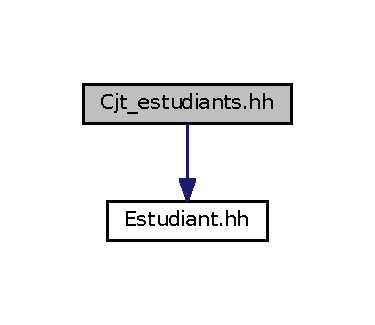
\includegraphics[width=180pt]{_cjt__estudiants_8hh__incl}
\end{center}
\end{figure}
\subsection*{Classes}
\begin{DoxyCompactItemize}
\item 
class \hyperlink{class_cjt__estudiants}{Cjt\+\_\+estudiants}
\begin{DoxyCompactList}\small\item\em Representa un conjunt d'estudiants ordenat per D\+N\+I. Es poden consultar i modificar els seus elements (de tipus \hyperlink{class_estudiant}{Estudiant}) donat un estudiant concret o per posicio a l'ordre. \end{DoxyCompactList}\end{DoxyCompactItemize}


\subsection{Descripció Detallada}
Especificació de la classe \hyperlink{class_cjt__estudiants}{Cjt\+\_\+estudiants}. 



Definició al fitxer \hyperlink{_cjt__estudiants_8hh_source}{Cjt\+\_\+estudiants.\+hh}.


\hypertarget{_estudiant_8hh}{\section{Referència del Fitxer Estudiant.\+hh}
\label{_estudiant_8hh}\index{Estudiant.\+hh@{Estudiant.\+hh}}
}


Especificació de la classe \hyperlink{class_estudiant}{Estudiant}.  


\subsection*{Classes}
\begin{DoxyCompactItemize}
\item 
class \hyperlink{class_estudiant}{Estudiant}
\begin{DoxyCompactList}\small\item\em Representa un estudiant amb D\+N\+I, que pot tenir nota. \end{DoxyCompactList}\end{DoxyCompactItemize}


\subsection{Descripció Detallada}
Especificació de la classe \hyperlink{class_estudiant}{Estudiant}. 



Definició al fitxer \hyperlink{_estudiant_8hh_source}{Estudiant.\+hh}.


\hypertarget{pro2__doxygen_8cc}{\section{Referència del Fitxer pro2\+\_\+doxygen.\+cc}
\label{pro2__doxygen_8cc}\index{pro2\+\_\+doxygen.\+cc@{pro2\+\_\+doxygen.\+cc}}
}
Inclou el graf de dependències per a pro2\+\_\+doxygen.\+cc\+:\nopagebreak
\begin{figure}[H]
\begin{center}
\leavevmode
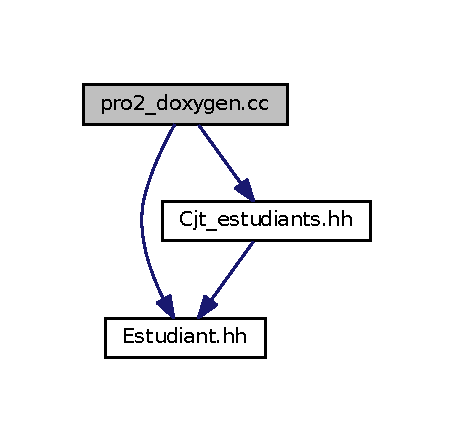
\includegraphics[width=218pt]{pro2__doxygen_8cc__incl}
\end{center}
\end{figure}
\subsection*{Funcions}
\begin{DoxyCompactItemize}
\item 
int \hyperlink{pro2__doxygen_8cc_ae66f6b31b5ad750f1fe042a706a4e3d4}{main} ()
\begin{DoxyCompactList}\small\item\em Programa principal. \end{DoxyCompactList}\end{DoxyCompactItemize}


\subsection{Documentació de les Funcions}
\hypertarget{pro2__doxygen_8cc_ae66f6b31b5ad750f1fe042a706a4e3d4}{\index{pro2\+\_\+doxygen.\+cc@{pro2\+\_\+doxygen.\+cc}!main@{main}}
\index{main@{main}!pro2\+\_\+doxygen.\+cc@{pro2\+\_\+doxygen.\+cc}}
\subsubsection[{main}]{\setlength{\rightskip}{0pt plus 5cm}int main (
\begin{DoxyParamCaption}
{}
\end{DoxyParamCaption}
)}}\label{pro2__doxygen_8cc_ae66f6b31b5ad750f1fe042a706a4e3d4}


Programa principal. 



Definició a la línia 20 del fitxer pro2\+\_\+doxygen.\+cc.


\begin{DoxyCode}
21 \{
22   \textcolor{comment}{// completeu amb el codi que volgueu}
23 \}
\end{DoxyCode}

%--- End generated contents ---

% Index
\newpage
\phantomsection
\addcontentsline{toc}{chapter}{Índex}
\printindex

\end{document}
